\documentclass{article}
\usepackage{tabularx}
\usepackage{amsmath}
\usepackage{here}
\usepackage{graphicx}
\usepackage[margin=2cm]{geometry}
\usepackage{cite}
\usepackage[final]{hyperref}
\usepackage{listings}
\hypersetup{
	colorlinks=true,
	linkcolor=blue,
	citecolor=blue,
	filecolor=magenta,
	urlcolor=blue         
}

\begin{document}

\title{TP01\\Introduction to parallel processing}
\date{01/03/23}
\maketitle

\begin{abstract}
	In this practical work, we will see how to convert a simple iterative process into a parallel process.
\end{abstract}


\section{Introduction}
First, generate the Visual Studio solution, compile it and run the TP01 program.
You'll find the source of the practical work by cloning this git repository:
\begin{lstlisting}
	https://github.com/robinfaurypro/GPGPU_ISIMA_2022-2023.git
\end{lstlisting}
The CMakeLists file is stored into the TP01 folder. Open a terminal on your working folder and use this cmake command:
\begin{lstlisting}
	cmake -G "Visual Studio 17 2022" -A x64 ..
\end{lstlisting}
If everything is going well, you can compile and run the TP01 executable. The application generate a grayscale image in 512 by 512 pixels.

\section{Image generation}
Colors in computer graphic are most often store into three channel RGB 8bits. That means 256 values per channel are available. This is a compromise between nice content and light storage. However, you can store image in a 16bit format (unsigned short) or 32bit (float). To manipulate the color, we usually convert it into normalized float value ($0 < color < 1$). In the same way, the coordinate are normalized ($\left\{
\begin{array}{rcr}
0<x<512 & \rightarrow & 0<u<1 \\
0<y<512 & \rightarrow & 0<v<1 
\end{array}
\right.$).
A GPU is efficient with float operation so it's a good idea to works with floating data.\\
The image\_data object store the interleaved data of the image. That mean the first value of the vector corresponding to the red value of a pixel, the second to the green and the third to the blue. Create a function to fill the image according to the picture. The u coordinate is assign to the red channel and the v coordinate to the green. The blue channel will be always zero.

\begin{figure}[H]
	\centering
	\reflectbox{\rotatebox[origin=c]{180}{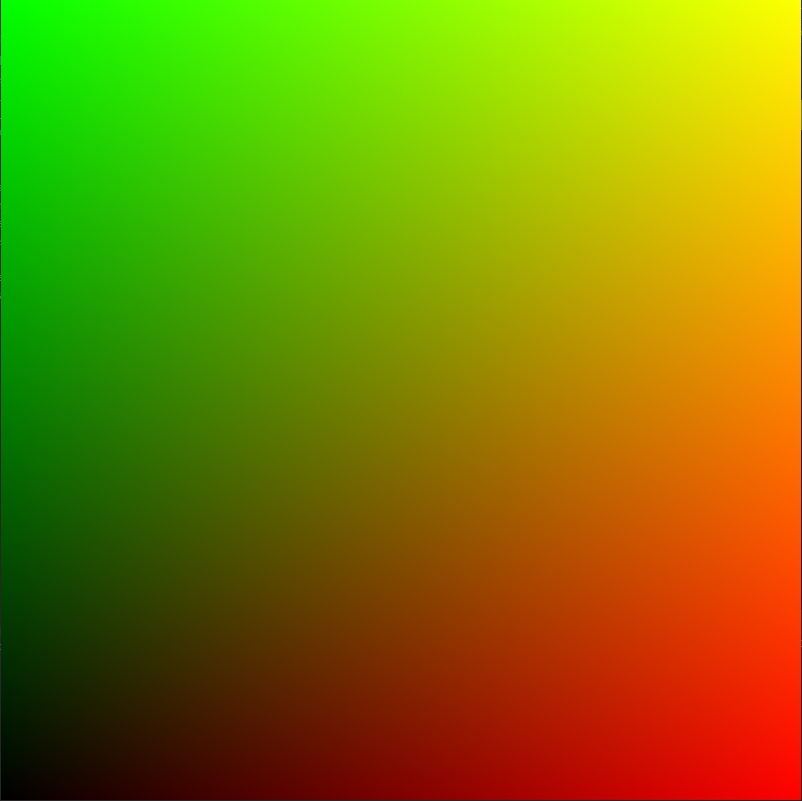
\includegraphics[scale=0.2]{figures/uv.png}}}
	\caption{UV of the image}
\end{figure}

Each coordinate can now be used to create an image with a disc on it.

\section{Critical path}
In GPGPU, the most important part is to identify the critical path. The critical path is the smallest piece of code that can be run in parallel. Find it and create a function "kernel" to isolate this path. You must review your function with the teacher.\\
We can now use std::thread to run in parallel our kernel. Take a look at your configuration to know how many logical processors do you have. Create one std::thread per logical processors. A std::thread need a function as input. Create a "dispatch" function that run the kernel for a subset of the image. 
\begin{lstlisting}
	std::thread t0(
		dispatch,
		startX,
		endX,
		startY,
		endY,
		width,
		height,
		iterationMax);
	//...
	t0.join();
	//...
\end{lstlisting}
At this step you need to set your buffer as a global variable if you want it to be shared between threads.

\section{The Mandelbrot set}
Let's try to have a more heavy parallel algorithm. The Mandelbrot set is the set of complex numbers $c$ for which the function
\begin{equation}
f_c(z) = z^2+c
\end{equation}
does not diverge when iterated from $z = 0+0i$.\\
As a reminder complex number multiplication is:
\begin{equation}
z_1*z_2 = (z_1.real*z_2.real-z_1.imag*z_2.imag) + (z_1.real*z_2.imag + z_1.imag*z_2.real)*i
\end{equation}
And the addition is:
\begin{equation}
z_1 + z_2 = (z_1.real + z_2.real) + (z_1.imag + z_2.imag)*i
\end{equation}
Create a struct Complex and provide an operator '+' and '*'. Provide also a function to compute the modulus of the complex too.\\
Choose a square size for the output image (for example 1024x1024) and create a buffer of float to store all RGB pixel. A pixel is three float from 0.f to 1.f.\\
Now the aim is to run the function $(1)$ for each pixel. First we need to convert each coordinate pixel to the complex plan.
\begin{lstlisting}
	Complex c(u, v);
\end{lstlisting}
We can run the function $(1)$ while the result don't diverge. We consider a complex number is outside of the [-2; 2] window is a divergent value. $iterationMax$ is the number max of "jump".
\begin{lstlisting}
	unsigned int cmp = 0u;
	while (modulus(z) < 2.f && cmp <= iterationMax) {
		z = z*z + c;
		++cmp;
	}
\end{lstlisting}
If cmp reach iterationMax that means the complex number chosen is part of the Mandelbrot set. We can set the color of this pixel to black. in the other case we can set the color to red. We can also use a gradient for a better result.
\begin{lstlisting}
	const float red = static_cast<float>(cmp)/static_cast<float>(iterationMax);
\end{lstlisting}

For your information the Mandelbrot set have a better look if $c$ is padded by $-1.5 - 0.5i$.

\begin{figure}[H]
	\centering
	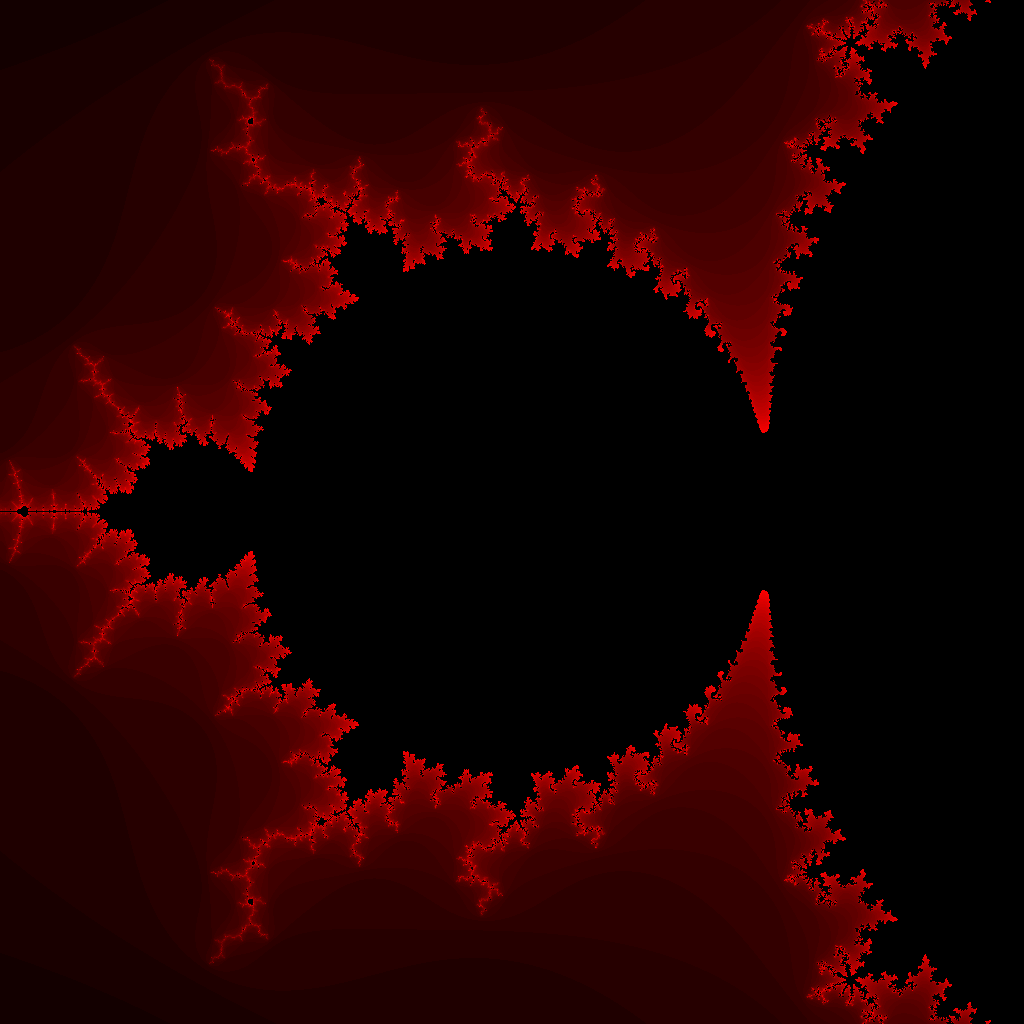
\includegraphics[scale=0.35]{figures/Mandelbrot.png}
	\caption{Mandelbrot set}
\end{figure}

\section{Julia set}
The Julia set is similar to the Mandelbrot set, but with a chaotic behaviour. That means iterationMax need to be increased if we want to compute the image. You can compute the fractal using those parameters:
\begin{itemize}
	\item z = u+v*i
	\item c = 0.292 + 0.015*i
	\item iterationMax = 400
\end{itemize}
\begin{figure}[H]
	\centering
	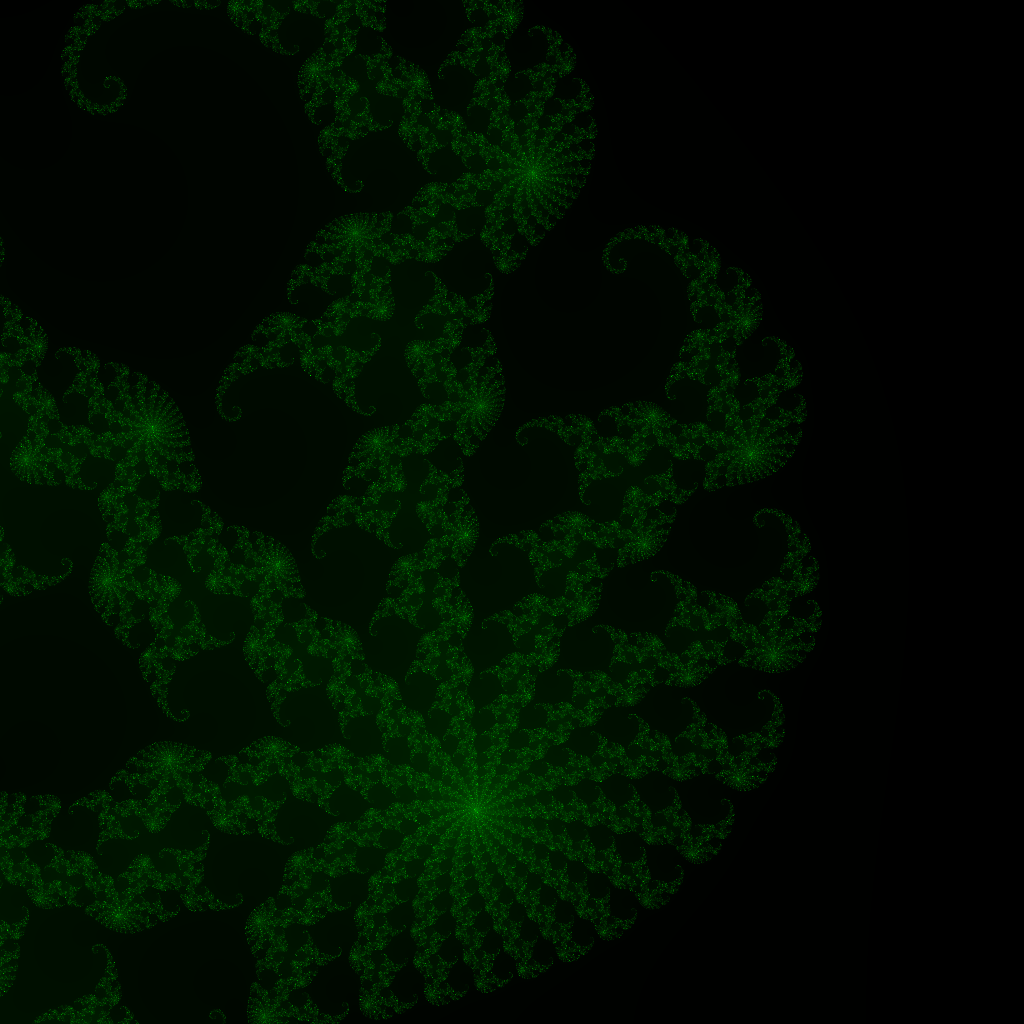
\includegraphics[scale=0.4]{figures/julia.png}
	\caption{Julia set}
\end{figure}

\end{document}